% Options for packages loaded elsewhere
\PassOptionsToPackage{unicode}{hyperref}
\PassOptionsToPackage{hyphens}{url}
%
\documentclass[
]{article}
\usepackage{lmodern}
\usepackage{amssymb,amsmath}
\usepackage{ifxetex,ifluatex}
\ifnum 0\ifxetex 1\fi\ifluatex 1\fi=0 % if pdftex
  \usepackage[T1]{fontenc}
  \usepackage[utf8]{inputenc}
  \usepackage{textcomp} % provide euro and other symbols
\else % if luatex or xetex
  \usepackage{unicode-math}
  \defaultfontfeatures{Scale=MatchLowercase}
  \defaultfontfeatures[\rmfamily]{Ligatures=TeX,Scale=1}
\fi
% Use upquote if available, for straight quotes in verbatim environments
\IfFileExists{upquote.sty}{\usepackage{upquote}}{}
\IfFileExists{microtype.sty}{% use microtype if available
  \usepackage[]{microtype}
  \UseMicrotypeSet[protrusion]{basicmath} % disable protrusion for tt fonts
}{}
\makeatletter
\@ifundefined{KOMAClassName}{% if non-KOMA class
  \IfFileExists{parskip.sty}{%
    \usepackage{parskip}
  }{% else
    \setlength{\parindent}{0pt}
    \setlength{\parskip}{6pt plus 2pt minus 1pt}}
}{% if KOMA class
  \KOMAoptions{parskip=half}}
\makeatother
\usepackage{xcolor}
\IfFileExists{xurl.sty}{\usepackage{xurl}}{} % add URL line breaks if available
\IfFileExists{bookmark.sty}{\usepackage{bookmark}}{\usepackage{hyperref}}
\hypersetup{
  pdftitle={Atividade x COVID},
  hidelinks,
  pdfcreator={LaTeX via pandoc}}
\urlstyle{same} % disable monospaced font for URLs
\usepackage[margin=1in]{geometry}
\usepackage{graphicx,grffile}
\makeatletter
\def\maxwidth{\ifdim\Gin@nat@width>\linewidth\linewidth\else\Gin@nat@width\fi}
\def\maxheight{\ifdim\Gin@nat@height>\textheight\textheight\else\Gin@nat@height\fi}
\makeatother
% Scale images if necessary, so that they will not overflow the page
% margins by default, and it is still possible to overwrite the defaults
% using explicit options in \includegraphics[width, height, ...]{}
\setkeys{Gin}{width=\maxwidth,height=\maxheight,keepaspectratio}
% Set default figure placement to htbp
\makeatletter
\def\fps@figure{htbp}
\makeatother
\setlength{\emergencystretch}{3em} % prevent overfull lines
\providecommand{\tightlist}{%
  \setlength{\itemsep}{0pt}\setlength{\parskip}{0pt}}
\setcounter{secnumdepth}{-\maxdimen} % remove section numbering

\title{Atividade x COVID}
\author{}
\date{\vspace{-2.5em}}

\begin{document}
\maketitle

\hypertarget{usando-dados-de-mobilidade}{%
\section{Usando dados de mobilidade}\label{usando-dados-de-mobilidade}}

\hypertarget{brasil}{%
\subsection{Brasil}\label{brasil}}

\includegraphics{activity_covid_files/figure-latex/unnamed-chunk-1-1.pdf}

\pagebreak

\hypertarget{regiuxe3o-sudeste}{%
\subsection{Região Sudeste}\label{regiuxe3o-sudeste}}

\includegraphics{activity_covid_files/figure-latex/unnamed-chunk-2-1.pdf}

\pagebreak

\hypertarget{regiuxe3o-sul}{%
\subsection{Região Sul}\label{regiuxe3o-sul}}

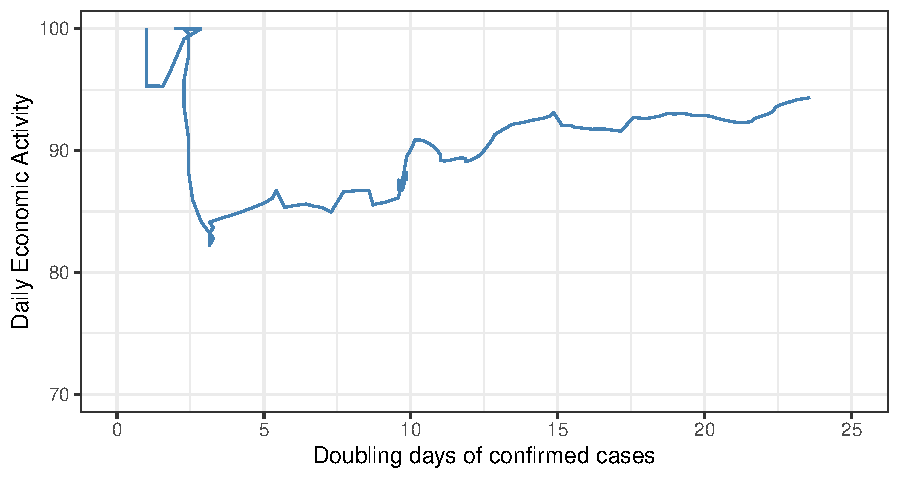
\includegraphics{activity_covid_files/figure-latex/unnamed-chunk-3-1.pdf}

\pagebreak

\hypertarget{regiuxe3o-centro-oeste}{%
\subsection{Região Centro-Oeste}\label{regiuxe3o-centro-oeste}}

\includegraphics{activity_covid_files/figure-latex/unnamed-chunk-4-1.pdf}

\pagebreak

\hypertarget{regiuxe3o-nordeste}{%
\subsection{Região Nordeste}\label{regiuxe3o-nordeste}}

\includegraphics{activity_covid_files/figure-latex/unnamed-chunk-5-1.pdf}

\pagebreak

\hypertarget{regiuxe3o-norte}{%
\subsection{Região Norte}\label{regiuxe3o-norte}}

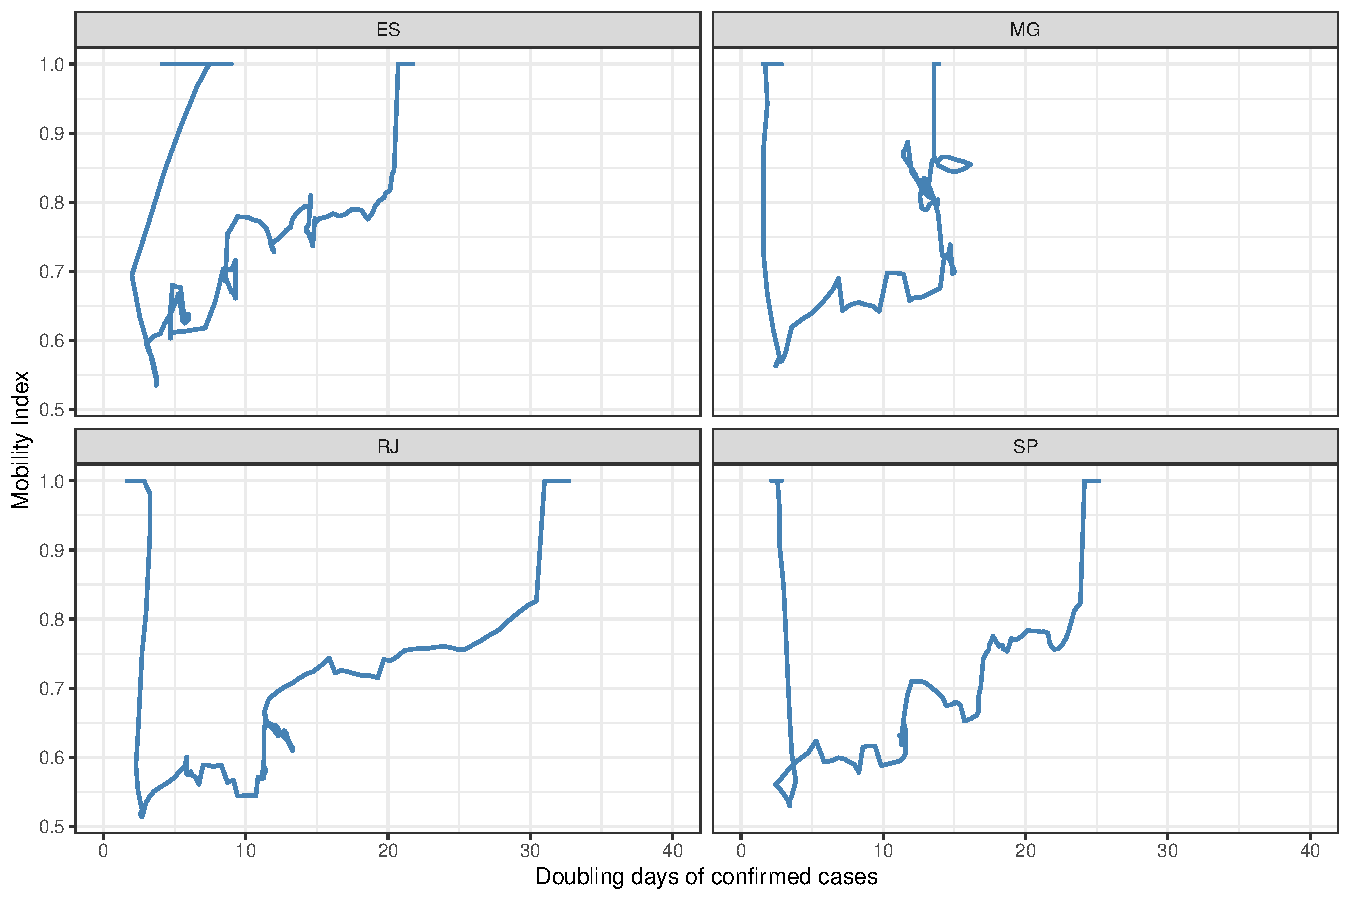
\includegraphics{activity_covid_files/figure-latex/unnamed-chunk-6-1.pdf}

\pagebreak

\hypertarget{usando-dados-de-energia}{%
\section{Usando dados de energia}\label{usando-dados-de-energia}}

Trocando os dados de mobilidade pela diferença percentual entre o
consumo de energia atual e o esperado.

Para definir o contrafactual, fazemos uma regressão para cada estado,
com os dados de 08/2018 até 02/2020, da seguinte forma:

\begin{equation}
\begin{split} \label{reg_energia}
\text{Consumo Diario}_{t} = \beta_0 & + \sum_{i=2}^{3} \psi_i D_{\text{ano}_{it}}+ \sum_{i=2}^{12} \delta_i D_{\text{mês}_{it}} + \sum_{i=2}^{7} \lambda_i D_{\text{dia da semana}_{it}} + \\
&\quad + \sum_{i=2}^{k} \theta_i D_{\text{feriado}_{it}} + \phi_1t + \phi_2t^2 + \epsilon_t
\end{split}
\end{equation}

A partir de \ref{reg_energia}, usamos os valores preditos para os dados
a partir de Março de 2020 como o esperado para o consumo de energia. A
diferença percentual mostrada nos gráficos abaixo se baseia nesses
valores.

\hypertarget{testando-o-fit}{%
\section{Testando o fit}\label{testando-o-fit}}

\hypertarget{regiuxe3o-sudeste-1}{%
\subsection{Região Sudeste}\label{regiuxe3o-sudeste-1}}

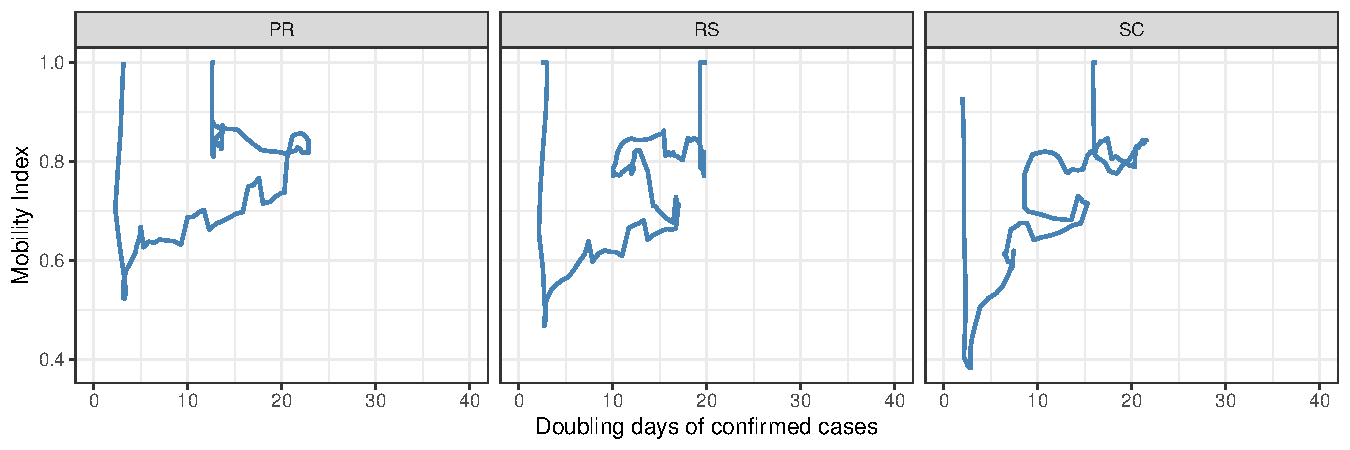
\includegraphics{activity_covid_files/figure-latex/unnamed-chunk-7-1.pdf}

\pagebreak

\textbf{Somente ACL}\\
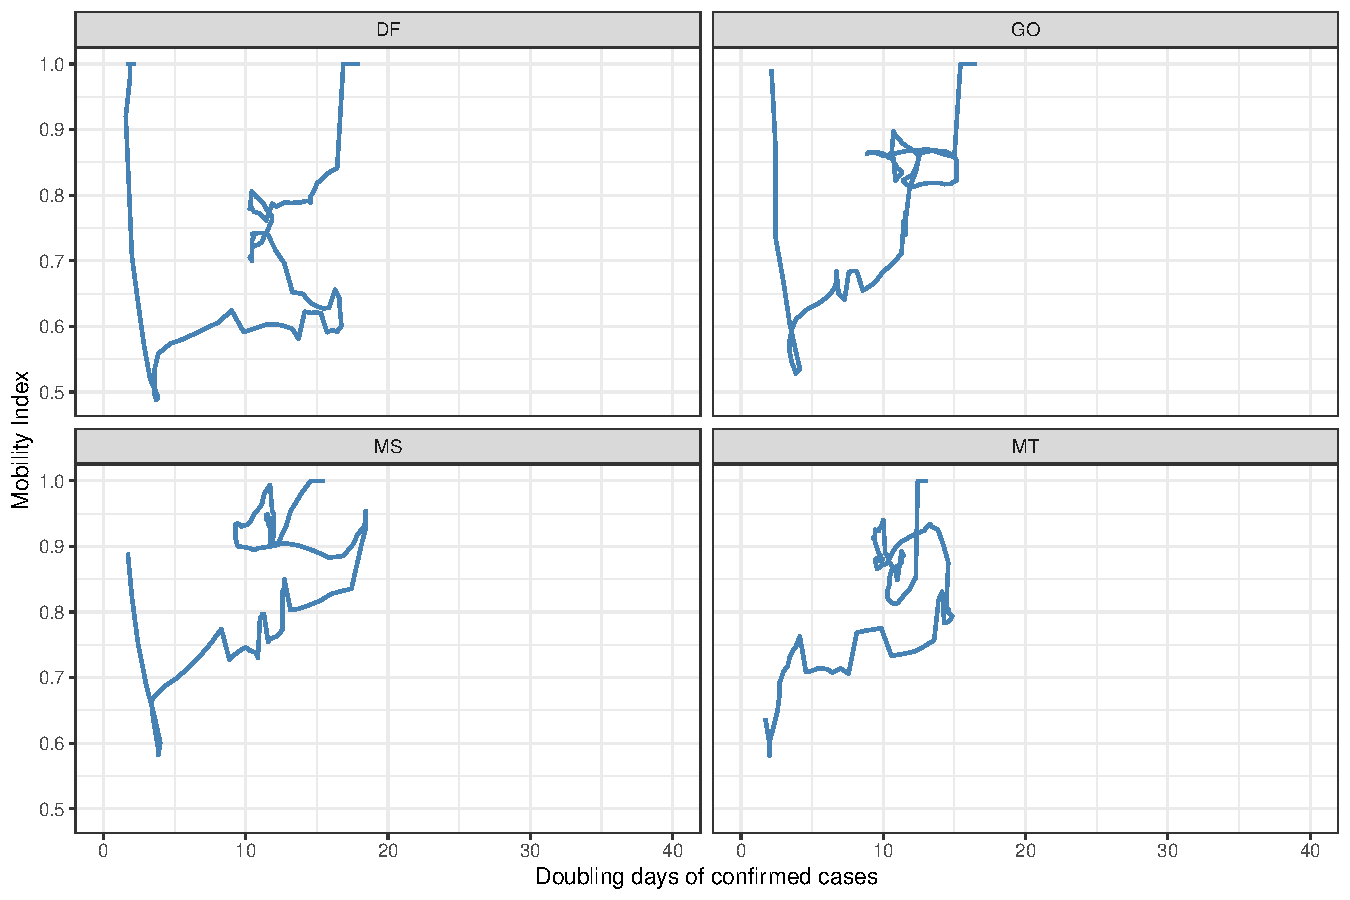
\includegraphics{activity_covid_files/figure-latex/unnamed-chunk-8-1.pdf}

\pagebreak

\hypertarget{regiuxe3o-sul-1}{%
\subsection{Região Sul}\label{regiuxe3o-sul-1}}

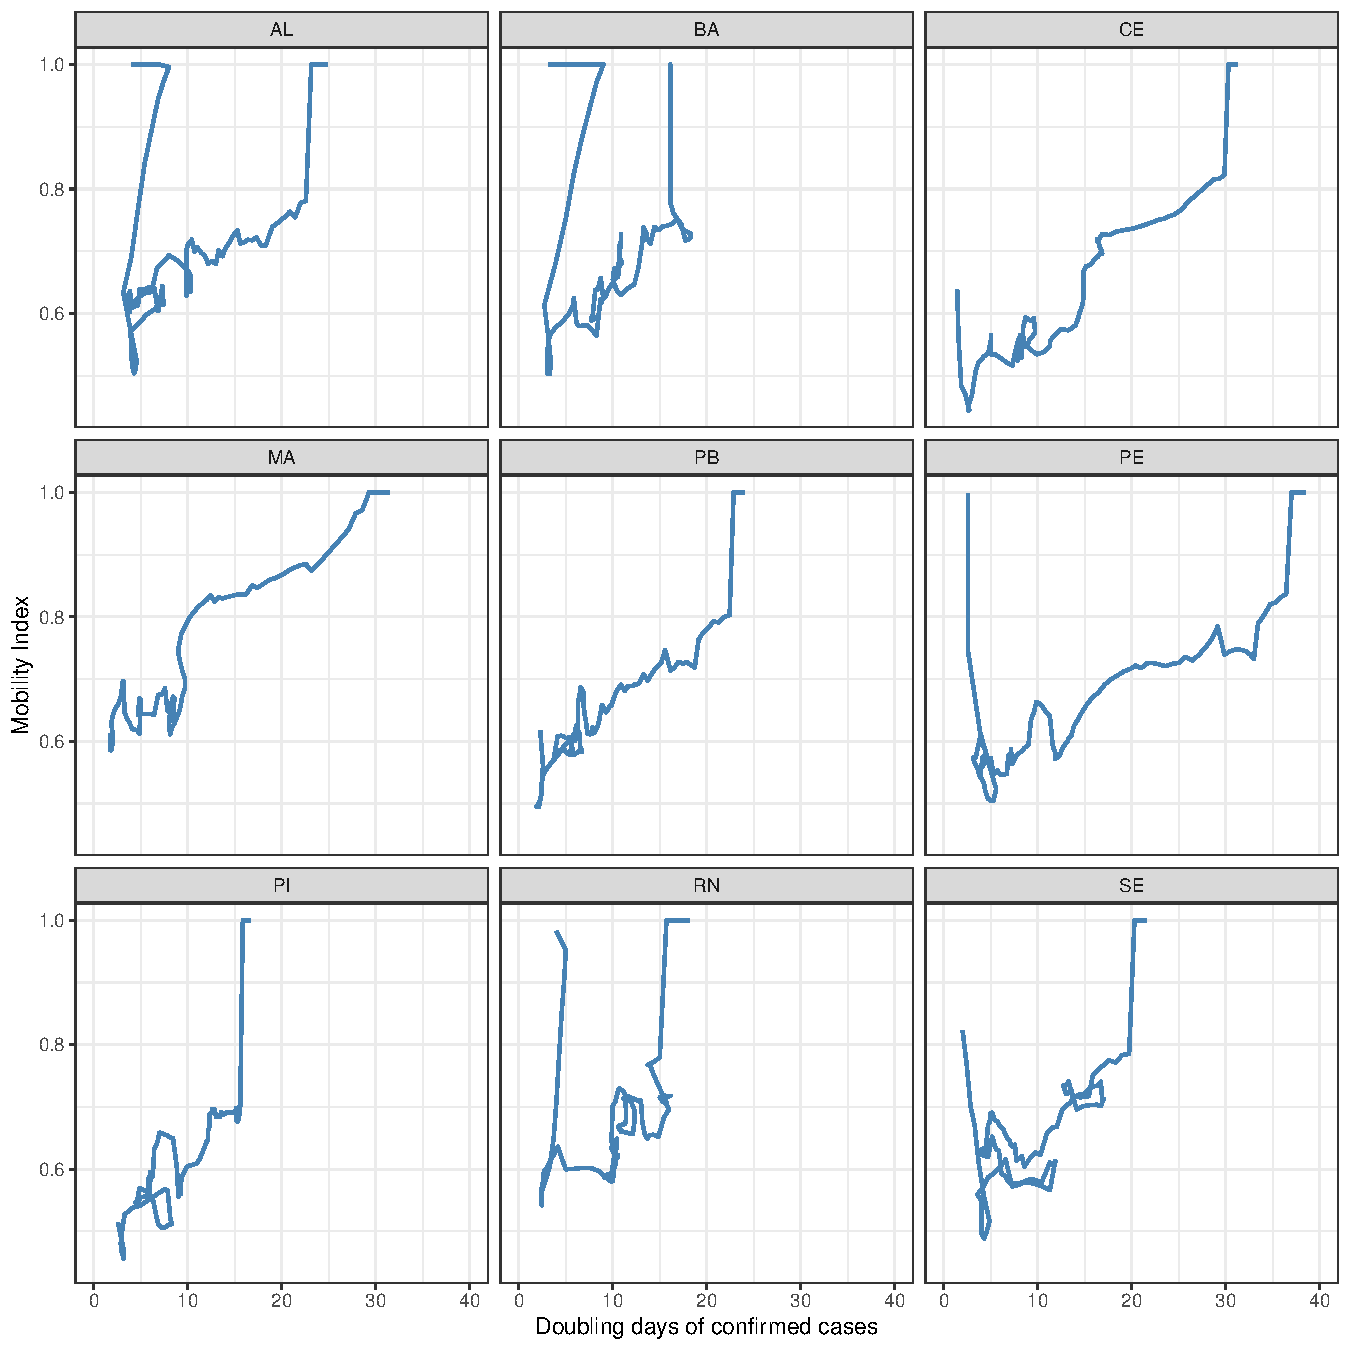
\includegraphics{activity_covid_files/figure-latex/unnamed-chunk-9-1.pdf}

\pagebreak

\textbf{Somente ACL}\\
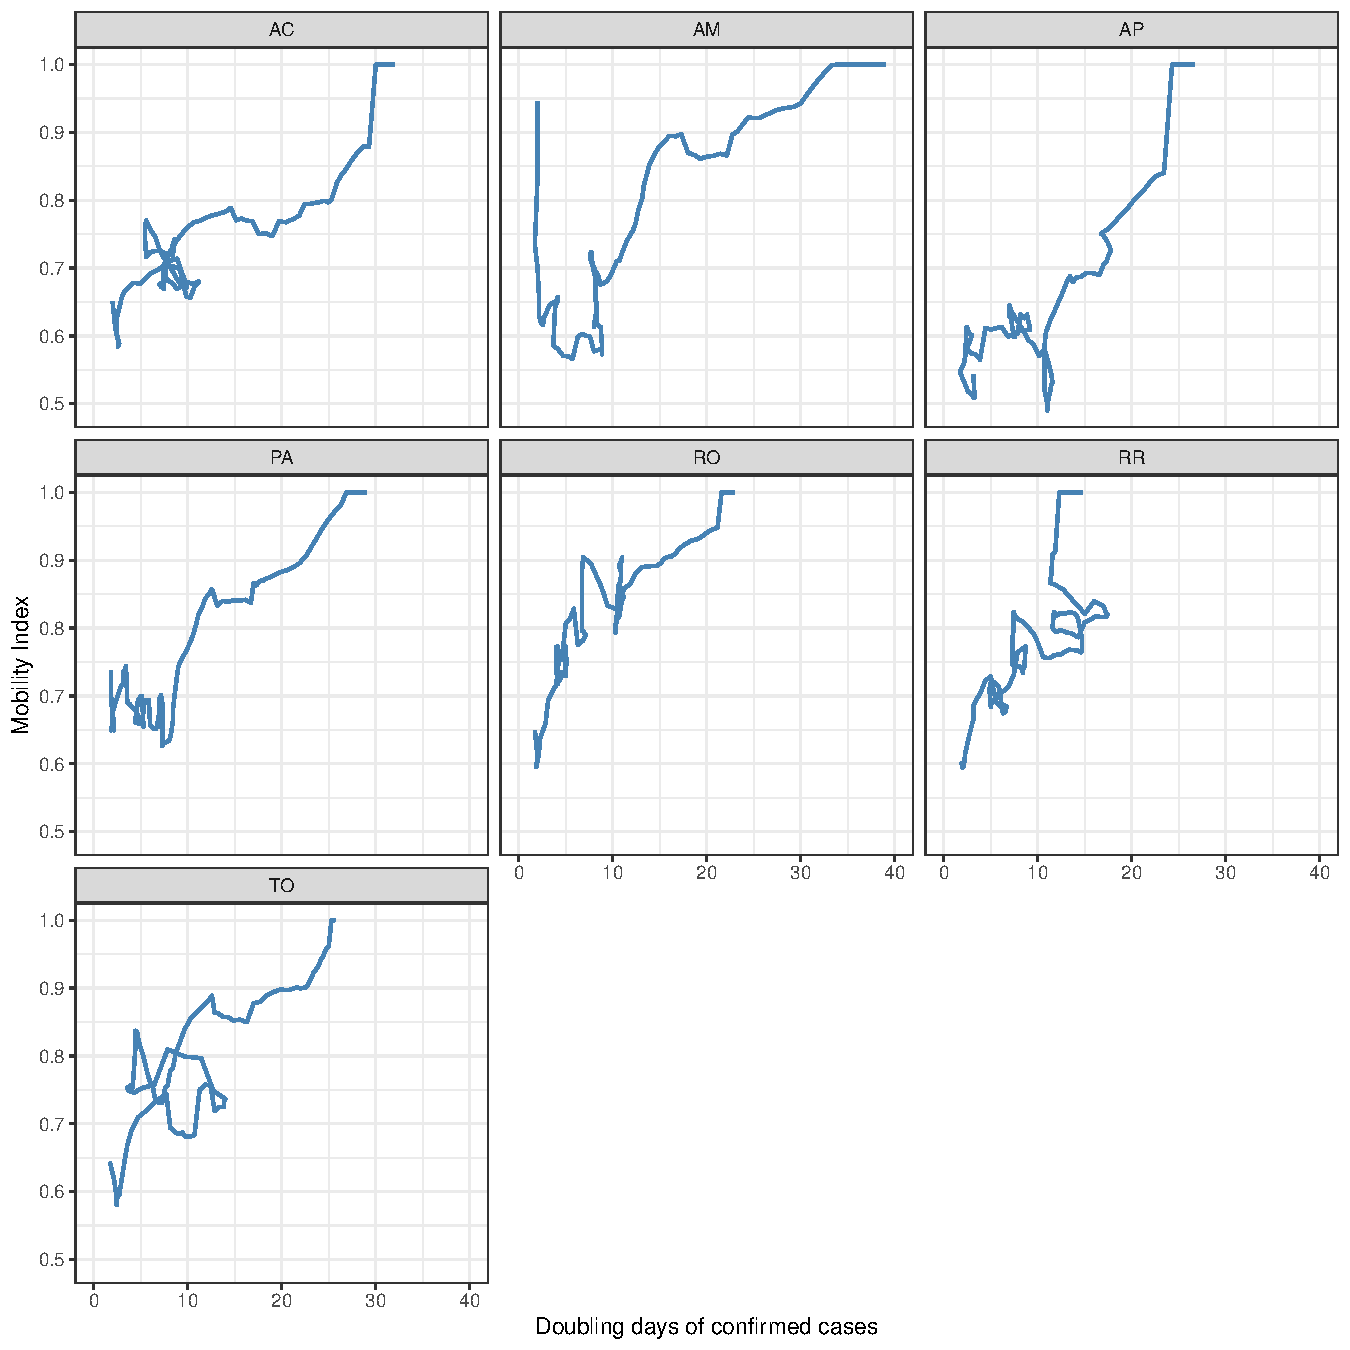
\includegraphics{activity_covid_files/figure-latex/unnamed-chunk-10-1.pdf}

\pagebreak

\hypertarget{regiuxe3o-centro-oeste-1}{%
\subsection{Região Centro-Oeste}\label{regiuxe3o-centro-oeste-1}}

\includegraphics{activity_covid_files/figure-latex/unnamed-chunk-11-1.pdf}

\pagebreak

\textbf{Somente ACL}\\
\includegraphics{activity_covid_files/figure-latex/unnamed-chunk-12-1.pdf}

\pagebreak

\hypertarget{regiuxe3o-nordeste-1}{%
\subsection{Região Nordeste}\label{regiuxe3o-nordeste-1}}

\includegraphics{activity_covid_files/figure-latex/unnamed-chunk-13-1.pdf}

\pagebreak

\textbf{Somente ACL}\\
\includegraphics{activity_covid_files/figure-latex/unnamed-chunk-14-1.pdf}

\pagebreak

\hypertarget{regiuxe3o-norte-1}{%
\subsection{Região Norte}\label{regiuxe3o-norte-1}}

\includegraphics{activity_covid_files/figure-latex/unnamed-chunk-15-1.pdf}

\pagebreak

\textbf{Somente ACL}\\
\includegraphics{activity_covid_files/figure-latex/unnamed-chunk-16-1.pdf}

\hypertarget{mudanuxe7a-para-o-previsto}{%
\section{Mudança para o previsto}\label{mudanuxe7a-para-o-previsto}}

\hypertarget{regiuxe3o-sudeste-2}{%
\subsection{Região Sudeste}\label{regiuxe3o-sudeste-2}}

\includegraphics{activity_covid_files/figure-latex/unnamed-chunk-17-1.pdf}

\pagebreak

\textbf{Somente ACL}\\
\includegraphics{activity_covid_files/figure-latex/unnamed-chunk-18-1.pdf}

\pagebreak

\hypertarget{regiuxe3o-sul-2}{%
\subsection{Região Sul}\label{regiuxe3o-sul-2}}

\includegraphics{activity_covid_files/figure-latex/unnamed-chunk-19-1.pdf}

\pagebreak

\textbf{Somente ACL}\\
\includegraphics{activity_covid_files/figure-latex/unnamed-chunk-20-1.pdf}

\pagebreak

\hypertarget{regiuxe3o-centro-oeste-2}{%
\subsection{Região Centro-Oeste}\label{regiuxe3o-centro-oeste-2}}

\includegraphics{activity_covid_files/figure-latex/unnamed-chunk-21-1.pdf}

\pagebreak

\textbf{Somente ACL}\\
\includegraphics{activity_covid_files/figure-latex/unnamed-chunk-22-1.pdf}

\pagebreak

\hypertarget{regiuxe3o-nordeste-2}{%
\subsection{Região Nordeste}\label{regiuxe3o-nordeste-2}}

\includegraphics{activity_covid_files/figure-latex/unnamed-chunk-23-1.pdf}

\pagebreak

\textbf{Somente ACL}\\
\includegraphics{activity_covid_files/figure-latex/unnamed-chunk-24-1.pdf}

\pagebreak

\hypertarget{regiuxe3o-norte-2}{%
\subsection{Região Norte}\label{regiuxe3o-norte-2}}

\includegraphics{activity_covid_files/figure-latex/unnamed-chunk-25-1.pdf}

\pagebreak

\textbf{Somente ACL}\\
\includegraphics{activity_covid_files/figure-latex/unnamed-chunk-26-1.pdf}

\hypertarget{relauxe7uxe3o-mobilidade-x-consumo-de-energia}{%
\section{Relação Mobilidade x Consumo de
Energia}\label{relauxe7uxe3o-mobilidade-x-consumo-de-energia}}

\hypertarget{regiuxe3o-sudeste-3}{%
\subsection{Região Sudeste}\label{regiuxe3o-sudeste-3}}

\includegraphics{activity_covid_files/figure-latex/unnamed-chunk-27-1.pdf}

\pagebreak

\textbf{Somente ACL}\\
\includegraphics{activity_covid_files/figure-latex/unnamed-chunk-28-1.pdf}

\pagebreak

\hypertarget{regiuxe3o-sul-3}{%
\subsection{Região Sul}\label{regiuxe3o-sul-3}}

\includegraphics{activity_covid_files/figure-latex/unnamed-chunk-29-1.pdf}

\pagebreak

\textbf{Somente ACL}\\
\includegraphics{activity_covid_files/figure-latex/unnamed-chunk-30-1.pdf}

\pagebreak

\hypertarget{regiuxe3o-centro-oeste-3}{%
\subsection{Região Centro-Oeste}\label{regiuxe3o-centro-oeste-3}}

\includegraphics{activity_covid_files/figure-latex/unnamed-chunk-31-1.pdf}

\pagebreak

\textbf{Somente ACL}\\
\includegraphics{activity_covid_files/figure-latex/unnamed-chunk-32-1.pdf}

\pagebreak

\hypertarget{regiuxe3o-nordeste-3}{%
\subsection{Região Nordeste}\label{regiuxe3o-nordeste-3}}

\includegraphics{activity_covid_files/figure-latex/unnamed-chunk-33-1.pdf}

\pagebreak

\textbf{Somente ACL}\\
\includegraphics{activity_covid_files/figure-latex/unnamed-chunk-34-1.pdf}

\pagebreak

\hypertarget{regiuxe3o-norte-3}{%
\subsection{Região Norte}\label{regiuxe3o-norte-3}}

\includegraphics{activity_covid_files/figure-latex/unnamed-chunk-35-1.pdf}

\pagebreak

\textbf{Somente ACL}\\
\includegraphics{activity_covid_files/figure-latex/unnamed-chunk-36-1.pdf}

\end{document}
